\chapter{Effective Transient Bounds and Finite Predictability}\label{ch:bounds}

Chapters~\ref{ch:gamma}--\ref{ch:select} show that every orbit eventually enters a rigid, exactly scaling regime governed by one prime. This chapter makes the word \emph{eventually} effective: from the finite data \((g_0,\gamma_0)\) of the initial state alone, it bounds how long the transient can last. The bounds depend on neither the size of the exponents nor of the starting value. Five results do this: a sharp bound on carries until the first reset (Theorem~\ref{thm:kappa}), a class-counting bound on the entry into the final cycle (Theorem~\ref{thm:entry}), a polynomial improvement (Theorem~\ref{thm:Kpoly}), a bound through changes of \(G\) (Theorem~\ref{thm:dynG}), and the registered scope of the whole programme (Theorem~\ref{thm:T73}).

\begin{definition}[Transient data]\label{def:transient}
Let \(f(a)=\lfloor a/4\rfloor+1\) and \(\kappa(a)=\min\{k:f^k(a)=1\}\) (\(\kappa(1)=0\)). For \(g\) odd let \(\mathcal P_g=\{p\nmid g:p^2<g\}\), and for \(g\) even \(\mathcal P_g=\{p\nmid g:p^2<4g\}\); by Theorem~\ref{thm:window}(c) these are the only primes that can carry after the first reset. Put
\begin{align*}
H(g)&=\prod_{p\in\mathcal P_g}(2o_p-1), & \Sigma&=\sum_{\mathcal P_g}o_p, & \omega&=\max_{\mathcal P_g}o_p, & \Phi&=\sum_{\mathcal P_g}(o_p-1),\\
K_{\mathrm{poly}}(g)&=(\Phi+1)\big(\Sigma+(\Sigma+1)(\omega+1)+1\big).
\end{align*}
A \emph{carry event} is a step with \(L'\ne L\); a \emph{reducing event} is a step with \(G'<G\) (Proposition~\ref{th:plateau-escape}); a \emph{segment} is a maximal run of constant \(G\). Carry events are counted, not collective-map steps; a plateau has at most \(4g\) steps (Proposition~\ref{th:plateau-escape}).
\end{definition}

\section{The reset-descent bound}

\begin{theorem}[Sharp reset-descent bound]\rec{F.T69}\scope{C}\label{thm:kappa}
In a segment of constant \(G=g\) (any \(g\), composite and even included) started at a state with \(\gamma=\gamma_0\), the first reset state is reached after at most \(\kappa(\gamma_0)\) carries, unless a reducing event ends the segment first. Moreover \(\kappa(a)=\min\{k:\ 3a\le2\cdot4^k+1\}\); equivalently \(\kappa(a)=k\) iff \(A_{k-1}<a\le A_k\) with thresholds \(A_k=(2\cdot4^k+1)/3=1,3,11,43,171,683,\dots\). Hence \(\kappa(a)\le\lceil\log_2a\rceil\), and \(\kappa(2)=1\), \(\kappa(10)=2\), \(\kappa(100)=4\), \(\kappa(1000)=6\), \(\kappa(10^6)=11\). The bound is attained at the eleven levels \(\kappa=1,\dots,11\): for each there are a prime \(g\) and a state with \(\gamma_0\) whose orbit needs exactly \(\kappa(\gamma_0)\) carries (Table~\ref{tab:kappa}). So the bound cannot be lowered at those levels; optimality at every other \(\gamma_0\) is not asserted.
\end{theorem}
\begin{proof}
By Theorem~\ref{thm:carrycomp}, a carry from a plateau that started at \(\gamma_s\ge1\) gives \(\gamma'\le\gamma_s/4+1\); as \(\gamma'\) is an integer, \(\gamma'\le f(\gamma_s)\). The map \(f\) is nondecreasing, so after \(k\) carries \(\gamma\le f^k(\gamma_0)\) (at the plateau start), and the plateau start is 1 as soon as \(f^k(\gamma_0)=1\). Between carries \(\gamma\) only grows (Theorem~\ref{thm:gamma}(c)), so \(\gamma=1\) can only occur directly after a carry or at the start.

\emph{Closed form.} Put \(A_0=1\), \(A_k=4A_{k-1}-1\), so \(A_k=(2\cdot4^k+1)/3\). Since \(f(a)\le A_{k-1}\iff\lfloor a/4\rfloor\le A_{k-1}-1\iff a\le4A_{k-1}-1=A_k\), induction gives \(f^k(a)=1\iff a\le A_k\) (\(f\ge1\), \(f(1)=1\)). So \(\kappa(a)\) is the least \(k\) with \(a\le A_k\), i.e. \(3a\le2\cdot4^k+1\). Finally \(a\le2^k\Rightarrow a\le A_k\) for \(k\ge1\) (as \(A_k\ge2^k\)), giving \(\kappa(a)\le\lceil\log_2a\rceil\).

\emph{Sharpness.} Table~\ref{tab:kappa} lists, for each \(\kappa\le11\), a reset-reaching state whose carry count was obtained by exact iteration of \(C\) (for \(\kappa\le8\)) and by the residue machine, validated against direct iteration, for larger \(\kappa\).
\end{proof}

\begin{table}[t]
\centering\small
\begin{tabular}{rrrr|rrrr}
\toprule
\(\kappa\) & \(g\) & \(\gamma_0\) & carries & \(\kappa\) & \(g\) & \(\gamma_0\) & carries\\
\midrule
1 & 61 & 2 & 1 & 7 & 151 & 10\,531 & 7\\
2 & 73 & 5 & 2 & 8 & 19 & 42\,663 & 8\\
3 & 61 & 37 & 3 & 9 & 11 & 173\,739 & 9\\
4 & 73 & 155 & 4 & 10 & 79 & 333\,226 & 10\\
5 & 193 & 345 & 5 & 11 & 103 & 1\,345\,610 & 11\\
6 & 31 & 1\,387 & 6 & & & &\\
\bottomrule
\end{tabular}
\caption{Witnesses that Theorem~\ref{thm:kappa} is sharp: in each case the state has \(\gamma=\gamma_0\) with \(\kappa(\gamma_0)=\kappa\) and the orbit needs exactly \(\kappa\) carries to reach \(\gamma=1\). The exponent states are listed in \texttt{witnesses.json} of the reproducibility package.}\label{tab:kappa}
\end{table}

\begin{figure}[t]
\centering
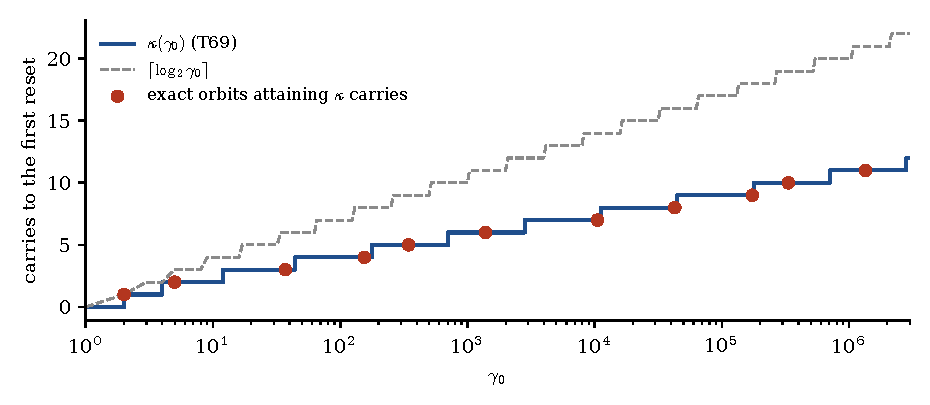
\includegraphics[width=0.9\linewidth]{figs/fig_kappa.pdf}
\caption{The reset-descent function \(\kappa(a)\) (steps) against \(\gamma_0\) on a logarithmic axis, with the witnesses of Table~\ref{tab:kappa} marked at their \(\gamma_0\): each witness lies exactly on the staircase, so the bound of Theorem~\ref{thm:kappa} is attained at each level \(1\le\kappa\le11\).}\label{fig:kappa}
\end{figure}

\emph{Scope.} \(\kappa\) counts carries, not steps. A plateau has at most \(4g\) steps, so the first reset is reached in at most \((\kappa(\gamma_0)+1)\,4g\) collective steps.

\section{The class-counting entry bound}

\begin{theorem}[Class-counting entry bound]\rec{F.T70}\scope{C}\label{thm:entry}
Let a segment have constant \(G=g\) and let \(s_0\) be its first reset state.
\begin{enumerate}[label=(\alph*),nosep]
\item If \(G\) stays \(g\) forever, the sequence of classes of the reset states \(s_0,s_1,\dots\) repeats within \(H(g)\) steps: the first repeated class occurs at index \(j\le H(g)\), the cycle is entered at an index \(i\le H(g)-1\), and from \(s_i\) on the orbit is purely periodic (\(x_{n+P}=\rho^2x_n\), Theorem~\ref{thm:closure}).
\item If the segment ends with a reducing event, it ends before the carry number \(H(g)\) after \(s_0\).
\item For prime \(g\) (more generally whenever Theorem~\ref{thm:certificate} applies) the entry state \(s_i\) is statically certified, (S3)--(S5), for the unique active prime \(r\).
\end{enumerate}
So the number of carries from the start of the segment to a certified state is at most \(\kappa(\gamma_0)+H(g)-1\), independent of the exponents. The certification clause (c) is proved for prime \(g\) only; the bound (a)--(b) holds for every \(g\).
\end{theorem}
\begin{proof}
After the first reset every carry is complete with \(M^2<g\) (for even \(g\), \(<4g\)) by Theorems~\ref{thm:carrycomp},~\ref{thm:window}, so only primes of \(\mathcal P_g\) change their exponent; all other exponents are constant. By Theorem~\ref{thm:predictor} the next reset state is a function of the class vector \((c_p(e_p))_{p\in\mathcal P_g}\) (Lemma~\ref{lem:class}), and a class has at most \(2o_p-1\) values (exact below saturation, then \(o_p\) residues), so there are at most \(H(g)\) class vectors.

(a) Among \(s_0,\dots,s_H\) two share a class; the first repeat has index \(j\le H\), so the entry is at \(i<j\le H\), i.e. \(i\le H-1\), and the closure principle (Theorem~\ref{thm:closure}) makes the orbit periodic from \(s_i\).

(b) If the segment lasted \(H\) carries after \(s_0\), the same pigeonhole argument would make it periodic, so no reducing event could occur (persistence of the next step is a function of the class, Lemma~\ref{lem:class}).

(c) In the cycle every carry recurs infinitely often, hence is a prime power (Theorem~\ref{thm:primepower}), and by Theorem~\ref{thm:dominance} only one prime \(r\) carries. \(r\) is saturated: its exponent rises in every period while its class returns, which is impossible for an unsaturated class (exact). The orbit from \(s_i\) carries only \(r\) and stays persistent: this is the hypothesis of the necessity half of Theorem~\ref{thm:certificate}, so (S3), (S4) hold, and (S5) is automatic for prime \(g\). The availability of coprime \(M\) does not depend on the phase of \(r\) (saturated), so (S4) holds at \(s_i\) as well as at the worst-case phase.
\end{proof}

\emph{Values.} \(H(11)=171\), \(H(31)=2\,655\), \(H(59)=21\,297\,195\); these are reproduced by the code of Appendix~\ref{app:algo}.

\section{The polynomial entry bound}

\begin{theorem}[Polynomial entry bound]\rec{F.T71}\scope{C}\label{thm:Kpoly}
In the setting of Theorem~\ref{thm:entry} (\(G=g\) from \(s_0\) on; \(g\) prime, or every prime factor of \(g\) larger than the squares of all carries, so that Theorem~\ref{thm:predictor} applies), the entry index and the exit index satisfy
\[
i\le K_{\mathrm{poly}}(g)=(\Phi+1)\big(\Sigma+(\Sigma+1)(\omega+1)+1\big),
\]
a cubic polynomial in the multiplicative orders instead of the product \(H(g)\). Values for \(g=11,31,59,101,197\):
\begin{align*}
K_{\mathrm{poly}}&=2\,688,\ 44\,928,\ 1\,243\,920,\ 10\,707\,144,\ 229\,237\,866,\\
H&=171,\ 2\,655,\ 21\,297\,195,\ 386\,149\,351,\ 1.78\cdot10^{15}.
\end{align*}
So \(K_{\mathrm{poly}}\) is the better bound from \(g\approx59\) on, and the minimum of the two is the bound. For \(g=211\): \(H(211)\approx2.4\cdot10^{13}\) and \(K_{\mathrm{poly}}(211)\approx1.1\cdot10^8\).
\end{theorem}
\begin{proof}
Call \(p\in\mathcal P_g\) \emph{saturated} if \(e_p\ge o_p-1\); saturation is monotone (exponents never decrease).

\emph{L1 (reduction).} The next carry \(M^\ast\) (Theorem~\ref{thm:predictor}) is either a pure power \(r^a\) of a saturated prime \(r\), or its prime support lies entirely among unsaturated primes. Indeed, if \(M=r^as\) (\(a\ge1\), \(s>1\) coprime to \(r\), \(r\) saturated) is available through \(d\), then \(d'=d\,r^{i-e_r-a}\) with \(i\equiv e_r+a\ (\mathrm{mod}\ o_r)\), \(0\le i\le e_r\), is a smaller divisor \(\equiv1\ (\mathrm{mod}\ g)\) with new part \(s<M\) (the argument of Theorem~\ref{thm:primepower}), so \(M\) is not minimal.

\emph{L2 (frozen competitor).} Availability of \(M\) with unsaturated support depends on the residues of the saturated primes only through the full subgroups \(\langle q\rangle\), and on the exact exponents of the unsaturated primes. Hence \(c_U:=\min\{\text{available }M\text{ with unsaturated support}\}\) is constant as long as no unsaturated exponent changes.

\emph{Epochs.} An \emph{epoch} is a maximal run of carries that are pure powers of saturated primes; it ends with a carry of unsaturated support (an \emph{epoch-ending} carry), or never. Such a carry raises \(\Phi_{\mathrm{cur}}=\sum_{\mathcal P_g}\min(e_p,o_p-1)\) by at least 1 (each prime of its support has \(e_p<o_p-1\)), so there are at most \(\Phi\) epoch-ending carries and at most \(\Phi+1\) epochs.

\emph{Inside an epoch} the saturated primes are independent odometers \(\Z/o_p\) with fixed tables \(\Abs_p\) (Theorems~\ref{thm:odometer},~\ref{thm:quotient}: the tables depend on the saturated set and on the frozen exact exponents), together with the frozen competitor \(c_U\) (if \(c_U\) ever wins, the epoch ends). Let \(p^\ast=\arg\min m_p\) over the saturated primes (Theorem~\ref{thm:minimax}).

\emph{Claim A.} Every saturated \(r\ne p^\ast\) fires at most \(|\Abs_r|\le o_r\) times in the epoch. After its first firing the phase of \(r\) lies in \(\Abs_r\), and each further firing moves it to the next element cyclically; within \(|\Abs_r|\) landings it lands on the element \(a^\ast\) before the largest gap, where its pending carry is \(m_r\). There \(c_{p^\ast}\le m_{p^\ast}<m_r\) (Theorem~\ref{thm:minimax}(i)), so \(r\) never fires again.

\emph{Claim B.} If \(p^\ast\) fires \(|\Abs_{p^\ast}|+1\) times in a row (no other prime, no \(c_U\) in between), the system returns to the state it had after the first of these firings, hence repeats forever: the class cycle has been entered. So in an epoch that is not the final periodic one, runs of consecutive \(p^\ast\)-firings have length \(\le|\Abs_{p^\ast}|\), and there are at most \(N_o+1\) such runs, where \(N_o\le\sum_{r\ne p^\ast}|\Abs_r|\le\Sigma\) is the number of non-survivor firings.

An epoch therefore contains at most \(N_o+(N_o+1)(|\Abs_{p^\ast}|+1)\le\Sigma+(\Sigma+1)(\omega+1)\) saturated carries before it ends or its cycle begins, plus the ending carry. Summing over at most \(\Phi+1\) epochs gives \(K_{\mathrm{poly}}\). The exit index obeys the same bound, since the carry sequence is deterministic until the window is violated.
\end{proof}

\begin{remark}[Numerical erratum to the source data sentence]\rec{F.E71}\scope{C}\label{rem:E71}
The data sentence of the source record quotes \(H\approx10^{15}\) and \(K_{\mathrm{poly}}\approx2\cdot10^8\) for \(g=211\); the exact values are \(H(211)=24\,165\,141\,422\,031\approx2.4\cdot10^{13}\) and \(K_{\mathrm{poly}}(211)=113\,903\,360\approx1.1\cdot10^8\) (the quoted figures match \(g=197\): \(H(197)\approx1.8\cdot10^{15}\), \(K_{\mathrm{poly}}(197)\approx2.3\cdot10^8\)). Only these two numerical expressions change; the theorem and its proof are unaffected. The values above were recomputed in exact integer arithmetic for this volume.
\end{remark}

\section{\texorpdfstring{The dynamic-\(G\) effective bound}{The dynamic-G effective bound}}

\begin{theorem}[Dynamic-\(G\) effective bound]\rec{F.T72}\scope{C}\label{thm:dynG}
Let \(x_0\) be any state (\(\Dx(x_0)\ne\emptyset\)) with \(G(x_0)=g_0\) and \(\gamma_0\). The orbit is a chain of segments \(g_0\supsetneq g_1\supsetneq\dots\supsetneq g_k\ge1\) (each \(g_{i+1}\mid g_i\)), and:
\begin{enumerate}[label=(\roman*),nosep]
\item the number of segments with \(G>1\) is at most \(\Omega(g_0)\) (prime factors with multiplicity);
\item at a reducing event \(g_i\to g_{i+1}\): \(\gamma_{i+1}=\frac{g_{i+1}}{g_i}\cdot\frac{\gamma_{\mathrm{before}}+1}{r^2}\), \(r=L'/L\ge1\), and \(\gamma_{\mathrm{before}}\le\gamma_i+4g_i\); hence \(\gamma_{i+1}\le g_{i+1}(\gamma_i+4g_i+1)/g_i\), a function of the finite data only;
\item segment \(i\) contains at most \(\kappa(\gamma_i)+H(g_i)-1\) \emph{carry events} (before its reducing event, or before the final class cycle is entered);
\item if the chain ends at \(G=1\) (regime~I), the tail to the cycle \(1\to2\to3\) takes at most \(4\kappa_3(t)\) steps, where \(\kappa_3(t)=\min\{k:f^k(t)\le3\}\), \(t=\gamma\) at the start of the tail;
\item hence the total number of carry events before the orbit is in its final class cycle is at most \(\mathcal R(g_0,\gamma_0)\), where \(\mathcal R(1,\cdot)=0\) and
\[
\mathcal R(g,\Gamma)=\kappa(\Gamma)+H(g)-1+\max_{g'\mid g,\ g'<g}\mathcal R\big(g',\lfloor g'(\Gamma+4g+1)/g\rfloor\big).
\]
This is explicit and computable from \((g_0,\gamma_0)\) alone.
\end{enumerate}
\emph{Qualification on units.} The principal bound (iii), (v) counts \emph{carry events}, not iterations of \(C\). The conversion to iterations uses three further estimates, each proved in this volume: a plateau has at most \(4g_i\) steps (Proposition~\ref{th:plateau-escape}), so segment \(i\) takes at most \((\text{carries}+1)\cdot4g_i+1\) steps; and the \(G=1\) tail takes at most \(4\kappa_3(t)\) steps, (iv). The theorem gives an \emph{explicit} bound; it does not give the exact transient time (Open Problem~\ref{op:exact}), and it is dominated by \(H(g_i)\) and astronomically larger than observed transients (Figure~\ref{fig:bounds}).
\end{theorem}
\begin{proof}
(i) \(\Dx(x)\subseteq\Dx(x')\) and \(G(x')\mid G(x)\) (Theorem~\ref{thm:mono}); a strictly decreasing divisibility chain \(g_0>g_1>\dots>g_k\ge2\) has \(\Omega(g_0)\ge\Omega(g_k)+k\ge k+1\).

(ii) \(x'=(\gamma+1)L^2/g\). At a reducing event \(G'=g'\), \(y'=g'x'=g'(\gamma+1)L^2/g\), so \(\gamma'=y'/L'^2=(g'/g)(\gamma+1)(L/L')^2\) (Theorem~\ref{thm:gamma}(a); \(L\mid L'\) because \(\Dx\subseteq\Dx'\)). Within a segment the plateau-start \(\gamma\) never rises (\(f(a)\le a\)), and each plateau adds at most \(4g\) to \(\gamma\) (Proposition~\ref{th:plateau-escape}), so \(\gamma_{\mathrm{before}}\le\gamma_i+4g_i\). With \(r\ge1\) this gives the stated inequality.

(iii) Theorem~\ref{thm:kappa} gives the carries to the first reset and Theorem~\ref{thm:entry} those after it: the segment is a constant-\(G\) run, so Theorems~\ref{thm:closure},~\ref{thm:window},~\ref{thm:carrycomp},~\ref{thm:predictor} apply to it verbatim, and since persistence of each step is a function of the class (Lemma~\ref{lem:class}), a segment that outlives \(H\) carries after its reset is periodic and never reduces. The step count follows from the plateau bound.

(iv) At \(G=1\) the state is \(x=s^2t\), \(\gamma=t\) squarefree (Theorems~\ref{thm:G-arith},~\ref{thm:regimeI}), and \(t\mapsto\mathrm{sqf}(t+1)\); the entry bound of Theorem~\ref{thm:regimeI} is \(4\kappa_3(t)\).

(v) Combine (ii)--(iv) and maximise over the possible chains: the next segment starts with some \(\gamma_{i+1}\le\lfloor g_{i+1}(\gamma_i+4g_i+1)/g_i\rfloor\) and \(\mathcal R(g',\cdot)\) is nondecreasing in its second argument.
\end{proof}

\begin{figure}[t]
\centering
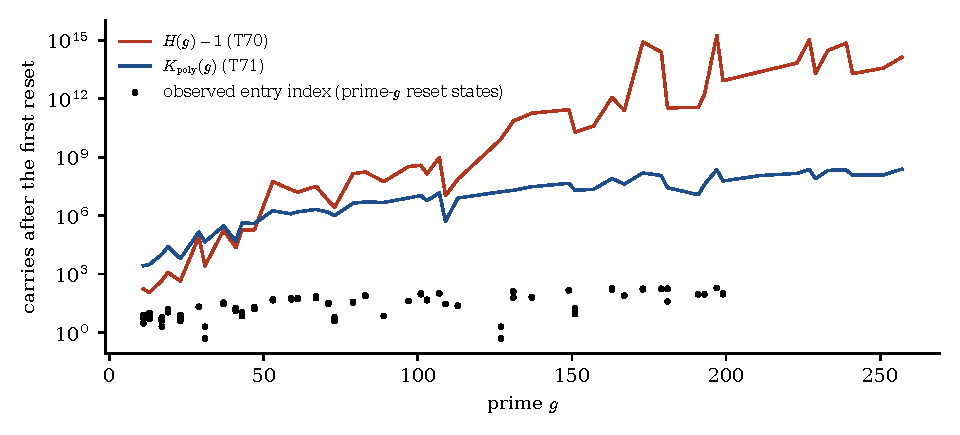
\includegraphics[width=0.97\linewidth]{figs/fig_bounds.pdf}
\caption{Observed versus certified transients. Each point is a random reset state at a prime \(g<200\), run exactly (\(n=150\) seeds); the vertical axis is the observed number of carries after the first reset before the cycle is entered. The curves are the bounds \(H(g)\) (Theorem~\ref{thm:entry}) and \(K_{\mathrm{poly}}(g)\) (Theorem~\ref{thm:Kpoly}). The largest observed index is 194 (\(g=197\)); the bounds exceed \(10^8\) there. They are worst-case guarantees, not predictions, and the gap between the points and the curves is Open Problem~\ref{op:exact}.}\label{fig:bounds}
\end{figure}

\section{Registered scope of the programme}

\begin{theorem}[Registered corrections and scope]\rec{F.T73}\scope{C}\label{thm:T73}
\begin{enumerate}[label=(E\arabic*),nosep]
\item \emph{Certification scope.} Theorem~\ref{thm:consequences}(a) is proved for prime \(g\). For composite or even \(g\) the hypothesis (S5) can fail while the orbit is persistent: in all six exact composite cycles tested (\(g=15,39,51,57,68,87\)) every reset state fails (S5). For such \(g\) the survivor exists (Theorem~\ref{thm:dominance}) and the class cycle is entered within \(H(g)\) carries (Theorem~\ref{thm:entry}(a)), but static certification as formulated in Theorem~\ref{thm:certificate} is not available (Open Problem~\ref{op:composite}).
\item \emph{Sharp constant.} The weaker form of the reset-descent bound, \(\gamma'\le\lfloor(\gamma+1)/4\rfloor\le\lfloor\gamma/2\rfloor\), loses a factor 2 per carry; the sharp statement is \(\kappa(\gamma_0)\approx\log_4\gamma_0\), and it is attained at the eleven levels of Table~\ref{tab:kappa} (Theorem~\ref{thm:kappa}).
\item \emph{Index.} The entry index is \(\le H-1\) (the first repeat is at \(\le H\)); Theorem~\ref{thm:Kpoly} supplies a bound that does not grow like a product over primes.
\item \emph{Effectiveness.} The question of a bound from an arbitrary seed before \(G\) stabilises is answered by Theorem~\ref{thm:dynG} as an explicit bound; the exact transient time remains open.
\end{enumerate}
\end{theorem}
\begin{proof}
(E1) is Theorem~\ref{thm:consequences} and the computation of Appendix~\ref{app:algo} for the six cycles; (E2)--(E4) are the content of Theorems~\ref{thm:kappa},~\ref{thm:entry},~\ref{thm:Kpoly},~\ref{thm:dynG}.
\end{proof}

\section{Finite predictability}

Combining the results of Chapters~\ref{ch:gamma}--\ref{ch:bounds}: for every initial state with \(\Dx(x_0)\ne\emptyset\),
\begin{enumerate}[nosep]
\item the orbit has a finite chain of values of \(G\) and eventually satisfies \(x_{n+P}=\rho^2x_n\) with \(\rho=p^s\) a prime power (Theorems~\ref{thm:closure},~\ref{thm:rho});
\item exactly one prime carries in the final regime (Theorem~\ref{thm:dominance}), and for prime \(g\) it is decided by a finite residue test (Theorems~\ref{thm:minimax}--\ref{thm:consequences});
\item the time to reach that regime is at most \(\mathcal R(g_0,\gamma_0)\) carry events, computable from \((g_0,\gamma_0)\) alone (Theorem~\ref{thm:dynG}).
\end{enumerate}
In this sense the asymptotics of the collective dynamics are \emph{effectively predictable}: existence (eventual exact scaling), structure (one prime, one carry word) and effectiveness (computable bounds on the transient) are all established, with the two scope qualifications stated in Theorems~\ref{thm:dynG} and~\ref{thm:certificate}.
